%#!platex -src-specials CategoryTheory.tex
\chapter{圏}\label{Categories}
\section{導入}
\index{けんろん@圏論|(}
{\bfseries 圏論とは何か?}まず例えるなら,圏論は(抽象的な)
{\bfseries 函数の代数\index{たいすう@代数}}\index{かんすう@函数|(}を調べ
る数学的な学問である,ということが出来るだろう.群論\index{くんろん@群論}が
集合の順列の仕組みや幾何学の対称性の概念を抽象化したものであるのと同様に,
圏論は幾つかの対象の間の函数の仕組みをかたどったものだ.

\begin{center}
 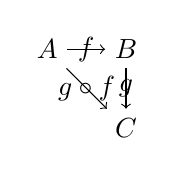
\begin{tikzpicture}
 \node (NA) {$A$};
 \node (NB) [right of=NA] {$B$};
 \node (NC) [below of=NB] {$C$};

 \draw [->]
  (NA) edge node {$f$} (NB)
       edge node[swap] {$g \circ f$} (NC)
  (NB) edge node {$g$} (NC);
 \end{tikzpicture}
\end{center}

圏論では,函数合成$g \circ f$を函数$g$と$f$の「積」 の一種と見て,函数
の集まりが成す「(抽象的な)代数\index{たいすう@代数}たち」を考えてゆく.圏とは単に,対象 $A, B,
C,\ldots $ と射 $ f: A \rightarrow B, g: B \rightarrow C,\ldots$ からなる
代数的構造で,射の合成について閉じていて更に幾つかの性質を満たすものであ
る.

圏論は抽象代数学の一分野であり,Felix Kleinの{\bfseries エルランゲン・
プログラム}の伝統の下で発明された.エルランゲン・プログラムとは,異なる
数学的構造を「適切な変換」の観点から捉えていこうという数学的な方法論であ
る.圏論の一般的な概念は,ある種の「構造を保つ変換」とそのような変換を許す
構造\index{こうそう@構造}の特徴付けを与える.

圏論の発展は,大まかに次のような経緯を辿ってきた.
\index{けんろん@圏論!のれきし@---の歴史}

\begin{description}
 \item[1945年] Eilenberg and Mac Lane\index{Mac Lane},
	    ``General theory of natural equivalence ''で圏の理論が初め
	    て定式化される
 \item[1940年代後半] 主に代数的トポロジー(特にホモロジー)や抽象代数の分
	    野で応用が見られる
 \item[1950年代] A. Grothendieck \index{Grothendieck}
	    らが代数幾何で圏論を用いて大きな成功を収める.
 \item[1960年代] F.W. Lawvere \index{Lawvere}らが圏を論理学
	    \index{ろんりかく@論理学}
	    に応用しはじめ,幾つかの深く驚くべき関連性を発見する.
 \item[1970年代] 既に計算機科学\index{けいさんきかかく@計算機科学},
	    言語学,認知科学,哲学など様々な分野
	    への応用が現れている.
\end{description}

このように,圏論は実に多岐にわたる応用範囲を誇っている.実際,集合論のよ
うに数学の汎用的な言語としても使えるということが明らかにされている.この
ような幅広い応用分野のため,圏論によって,例えば論理学と幾何学などの異な
る分野間の関連性が明らかになる,といったことがよく起こる.例えば,重要な
概念である{\bfseries 随伴函手}\index{すいはんかんしゆ@随伴函手}(adjoint
functor)の概念は,論理学においては存在量化子に対応し,位相幾何学では連続
関数に沿った像の操作に対応している.圏論的な視点に立てば,実はこれらは本
質的に同じ操作であるということが明らかになる.

随伴函手の概念は,読者がこの本を離れて他のより発展的な本で学ぶべき主な事
項のひとつだ.随伴の概念は,厳密に圏論的な概念でありながら後に第一級の道
具であることが明らかにされた.随伴は連続関数に比肩しうる概念である.

実際,圏論の発明者のひとりによれば,位相空間が連続函数についての洞察の為
に発明されたように,圏は函手を定義するために発明された.函手の概念は自然
変換(natural transformation)\index{しせんへんかん@自然変換}
を定義するために現れた,と話は続く.
さらに続けて,自然変換は随伴を定義する為のものであるといったほうが良いか
もしれない:
\begin{center}
 圏\index{けん@圏}\\
 函手\index{かんしゆ@函手}\\
 自然変換\\
 随伴\index{すいはん@随伴}
\end{center}
これは実際,この本の良い要約になっている.

本題に入る前に,何故圏論がそれほどまでに幅広い応用範囲を誇っている
のかについて説明させて貰いたい.さて,圏論とは函数の抽象的な理論であるこ
とは既に述べた.そうなれば,答えは簡単だ.

\begin{quote}
 {\bfseries いたるところ函数あり!}
\end{quote}

そして函数あるところ圏がある.本当のところ,圏論は「抽象函数論」とか,或
いは「アーチェリー」といったほうがもっと良いのかもしれない\footnote{訳注:
圏論では射(arrow)=矢を沢山扱うから,という洒落であろう}.
\index{けんろん@圏論|)}

\section{集合の函数}
\label{sec:functions of sets}
\index{しゆうこう@集合}
\index{しやそう@写像|(}
まず,集合の間の写像について見ていく.ここでは集合とは何かとか写像とは
何かとかの説明はしないで,そういった概念を扱えるだけ知識を仮定する.
それらは実際圏論を用いて定義することも出来るのだが,それはここでの目的で
はない.

集合$A$から$B$への写像$f$は次のように書く:
\[
 f: A \rightarrow B
\]
陽にいえば,これは$A$ の任意の元に対して$f$ の値が定義されており,その
結果は全て$B$に属す,ということである.集合論の言葉を使えば,

\[
 \mathrm{range}(f) \subseteq B
\]
ということである.

更に,写像$g: B \to C$があったとき,
\begin{center}
 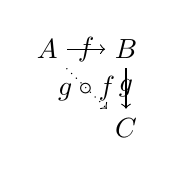
\begin{tikzpicture}
  \node (A) {$A$};
  \node (B) [right of=A]{$B$};
  \node (C) [below of=B]{$C$};
  \draw[->]
   (A) edge node {$f$} (B)
   (B) edge node {$g$} (C)
   (A) edge [dotted] node [swap] {$g \circ f$} (C);
 \end{tikzpicture}
\end{center}
\index{すしき@図式!かかん@可換---}
合成写像\index{こうせい@合成!しやぞう@---写像}
$g \circ f : A \to C$ は次で与えられる:
\begin{align}
 (g \circ f)(a) = g(f(a))\ \ \  a \in A \label{compdef}
\end{align}
こうして定義された写像合成の演算「$\circ$」は結合的である.写像
$h: C \to D$ があるとする.

\begin{center}
 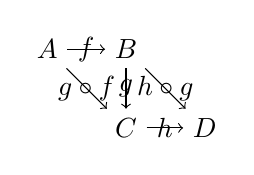
\begin{tikzpicture}
  \node (A) {$A$};
  \node (B) [right of=A] {$B$};
  \node (C) [below of=B] {$C$};
  \node (D) [right of=C] {$D$};

  \draw[->]
   (A) edge node{$f$} (B)
       edge node [swap] {$g \circ f$} (C)
   (B) edge node {$h \circ g$} (D)
       edge node {$g$} (C)
   (C) to node [swap] {$h$} (D);            
 \end{tikzpicture}
\end{center}
このとき,上図のように$h \circ g$と$g \circ f$が定義出来る.特に上図に示
された二つの写像$(h\circ g) \circ f$と$h \circ (g \circ f)$を見比べてみ
よう.定義から,これら二つの写像は常に等しいことがわかる.
\[
 (h\circ g) \circ f = h \circ (g \circ f)
\]
何故ならば,$(\ref{compdef})$より任意の $a \in A$ に対し,
\[
 ((h\circ g) \circ f)(a) = h(g(f(a))) = (h \circ (g \circ f))(a)
\]
が成立するからである.

ところで,上の議論は,二つの写像が等しいということの定義を
与えてもいる.\index{しやそう@写像!のとうちせい@---の同値性}
即ち,どんな引数に対しても同じ値を取れば二つの函数
は等しいと見做すのである.

最後に注意しておきたいのは,どんな集合$A$についても恒等写像
\index{しやそう@写像!こうとう@恒等---}
\[
 1_A : A \to A
\]
があって,次が成立していることである:
\[
 1_A(a) = a
\]

これらの恒等写像は,合成演算$\circ$について代数\index{たいすう@代数}的な
意味で「単位元」として振る舞う.つまり,任意の$f: A \to B$について,
\[
 f \circ 1_A = f = 1_B \circ f
\]
が成立している.

\begin{center}
 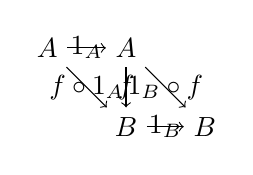
\begin{tikzpicture}
  \node (A1) {$A$};
  \node (A2) [right of=A1] {$A$};
  \node (B1) [below of=A2] {$B$};
  \node (B2) [right of=B1] {$B$};

  \draw[->] (A1) to node {$1_A$} (A2);
  \draw[->] (A2) to node {$1_B \circ f$} (B2);
  \draw[->] (A1) to node [swap]{$f \circ 1_A$} (B1);
  \draw[->] (B1) to node [swap]{$1_B$} (B2);
  \draw[->] (A2) to node {$f$} (B1);
 \end{tikzpicture}
\end{center}

抽象的な函数の概念として考察していきたいものは,合成写像や恒等写像などこ
れらでで全てである.なので,これらの物以外はいうなれば「捨象」して
しまって,次節の定義を得る.
\index{しやそう@写像|)}
\index{かんすう@函数|)}

\section{圏の定義}
\begin{definition}
 {\bf 圏}\index{けん@圏|textit}は次の要素からなる.
 \begin{itemize}
  \item {\bfseries 対象}\index{たいしよう@対象|textit}:$A,B,C,\ldots$
  \item {\bfseries 射}\index{しや@射|textit}:$f,g,h,\ldots$
  \item 任意の射$f$に対して,{\bfseries ドメイン}(域,始域;{\itshape
	domain})\index{とめいん@ドメイン|textit}
	\index{いき@域|see{ドメイン}}
	\index{しいき@始域|see{ドメイン}},{\bfseries コドメイン}
	\index{ことめいん@コドメイン|textit}(余域,終域;
	{\itshape codomain})
	\index{よいき@余域|see{コドメイン}}
	\index{しゆういき@終域|see{コドメイン}}と呼ばれる対象,
	\[
	 \dom(f), \cod(f)
	\]
	が与えられている.特に$A = \dom(f), B = \cod(f)$ のとき,
	\[
	 f : A \to B
	\]
	と書く.
  \item 射 $f: A \to B$ と $g: B \to C$ があるとき,即ち,
	\[
	 \cod(f) = \dom(g)
	\]
	なる二つの射があるとき,$f$ と $g$ の{\bfseries 合成射}
	\index{こうせい@合成|textit}
	\[
	 g \circ f : A \to C
	\]
	が与えられている.
  \item 任意の対象 $A$ について,{\bfseries 恒等射}
	\index{こうとうしや@恒等射|textit}
	\[
	 1_A : A \to A
	\]
	が存在する.
 \end{itemize}
 
 これらの要素は次の条件を満たさなくてはならない:
 \begin{itemize}
  \item 結合律\index{けつこうりつ@結合律|textit}:任意の
	$f: A \to B,\; g: B \to C,\; h: C \to D$ について,
	\[
	 h \circ (g \circ f) = (h \circ g) \circ f
	\]
  \item 単位律\index{たんいりつ@単位律|textit}:任意の $f : A \to B$ について,
	\[
	 f \circ 1_A = f = 1_B \circ f
	\]
 \end{itemize}
\end{definition}

これらの条件を満たすものは何でも圏であり,すぐに豊富な例を見てい
く.強調しておきたいのは,第\ref{sec:functions of sets}節とは異なり,対象
は集合でなくてもよいし,射も写像でなくてよいということである.この意味で,
圏は函数,つまり「射」(「モルフィズム」
\index{もるふいすむ@モルフィズム|textit}と呼ばれるこ
ともある)とその合成演算のなす{\bfseries 抽象}代数である.群論に詳しけれ
ば,圏が群\index{くん@群}のある種の一般化になっている事に気付くかもしれない.

\section{圏の例}
\label{Sec:Example of Categories}
\begin{enumerate}
 \item 集合と写像からなる圏 $\Sets$ \index{Sets@$\Sets$}は既に
       第\ref{sec:functions of sets}節で見た.他に全ての有限集合とその間
       の写像からなる圏
       \[
	\Sets_{\rm fin}
       \]
       \index{Sets fin@$\Sets_{\rm fin}$}がある.

       実際,このように対象となる集合や射となる写像を制限した圏は多くあ
       る.例えば,有限集合を対象,単射写像(1対1写像)
       \index{しやそう@写像!たんしや@単射---}を射とするものを考え
       ると,単射どうしの合成は再び単射となり,恒等写像は単射なので
       これも圏になる.

       では,集合を対象とし,各点の逆像の元が高々二つである写像を射とし
       た場合,これは圏になるだろうか?即ち,任意の $b \in B$ に対して,
       部分集合
       \[
	f^{-1}(b) \subseteq A
       \]
       が一つではなく高々二つの元を持つような写像$f$を射とした場合はどう
       だろうか?更に,$f^{-1}(b)$の元の個数が有限個とした場合,無限個と
       した場合はそれぞれどうだろうか?このように,集合と写像を制限した
       圏は実に沢山存在する.
 \item 数学にでしばしば見られる圏のもうひとつ例は,{\bfseries 構造の
       入った集合}
       \index{しゆうこう@集合!こうそうのはいつた@構造の入った---}か
       らなる圏である.つまり,さらに「構造」を持った集合
       とそれを「保存する」写像からなる圏である.そうした性質はそれぞれ
       独立に確かめることが出来るものとする.その種の例としては,以下の
       例がわかりやすいかもしれない:
       \begin{itemize}
	\item 群\index{くん@群}と群の準同型
	\item ベクトル空間と線型写像\index{しやそう@写像}
	\item グラフ\index{くらふ@グラフ}とグラフ準同型
	\item 実数の集合$\R$と連続函数
	      \index{かんすう@函数!れんそく@連続---}$\R\to\R$
	\item 開部分集合 $U \subseteq \R$ とその上で定義された連続函数
	      $f : U \to V \subseteq \R $
	\item 位相空間\index{いそうくうかん@位相空間}と連続写像
	      \index{しやそう@写像!れんそく@連続---}
	\item 可微分多様体と滑らかな写像
	\item 自然数の集合 $\N$ と任意の再帰函数$\N \to \N$.または,
	      連続函数の例と同じように,$U\subseteq\N$で定義された部分再
	      帰函数.\index{かんすう@函数!さいき@再帰---}
	\item 半順序集合と単調写像\index{しやそう@写像!たんちよう@単調---}
       \end{itemize}
       上のうち幾つかはよくわからないかもしれないが,特に気にする必要は
       ない.後ほど,上のうち幾つかを取り上げて詳しくみていく.次の例
       では,一番最後の例を取り上げてみよう.
 \item 半順序集合(partially ordered set),あるいは略して{\itshape poset}
       \index{poset|textit} とは,次を満たす二項関係$a \leq_A b$が入った
       集合のことである.任意の$a,b,c\in A$について,
       \begin{description}
	\item[反射律] $a\leq_A a$
	\item[推移律] $a\leq_A b$ かつ $b \leq_A c $ ならば $a \leq_A c$
	\item[反対称律] $a \leq_A b$ かつ $b \leq_A a$ ならば $a=b$
       \end{description}

       例えば,実数全体$\R$は通常の順序 $x \leq y$ によって{\bfseries 線
       型}な順序が入った poset となる.即ち,任意の $x, y$ に対して $x
       \leq y$ か $y \leq x$ かのどちらかが常に成立している.

       poset A から poset B への射は単調写像
       \[
	m : A \to B
       \]
       である.単調写像とは,任意の $a, a' \in A$ について,
       \[
	a \leq_A a'\; \text{ならば}\; m(a) \leq m(a')
       \]
       が成り立つような写像のことである.
       これを圏とするためにはどうすればいいだろうか?まず $1_A : A \to
       A$ が単調であることを確かめなくてはならないが,明らかに $a \leq_A
       a'$ ならば $a \leq_A a'$ が成り立つのでこれは正しい.
       また,$f:A \to B$ と $g: B \to C$ が単調のとき,$g \circ f : A
       \to C $も再び単調写像となることも確かめなくてはならないが,これも
       成立する.何故なら,$a \leq a'$ ならば $f(a) \leq f(a')$,
       $f(a) \leq f(a')$ ならば $g(f(a)) \leq g(f(a'))$ が成立し,従って
       $(g\circ f)(a) \leq (g\circ f)(a')$ が成立するからである.
       以上より,poset と単調写像は圏$\Pos$\index{Pos@$\Pos$}をなす.
 \item 今まで見てきた例は,{\bfseries 具体圏}\index{けん@圏!くたい@具体---}
       ({\itshape concrete category})と呼ばれる類のものだった.
       つまり,直感的には(何らかの構造を持った)集合を対象とし,その間の(構造を
       保つ)写像を射とする圏であった(この概念が必ずしも完全なも
       のではないことを後で見る;注意1.7を参照).
       しかし,圏論とは一体どういったものであるかを理解するひとつの方法
       は「元を使わずに考える」ことであり,元を射に置き換えて考えること
       である.そこで,このような考え方が単なる選択肢ではなく本質的な役割
       を果す例を見てみよう.

       圏$\Rel$ \index{Rel@$\Rel$}を対象を集合,射を二項関係
       \index{かんけい@関係}とする圏とする.つまり,射 $f: A\to B$は任意
       の部分集合 $f \subseteq A \times B$ である.集合 $A$ 上の恒等射は,
       恒等関係\index{かんけい@関係!こうとう@恒等---},
       \[
	1_A = \set{(a,a) \in A \times A | a \in A} \subseteq A \times A
       \]
       である.
       $R \subseteq A \times B$ と $S \subseteq B \times C$ が与えられた
       とき,その合成 \index{かんけい@関係!こうせい@合成---}
       $S \circ R$ は次で定義される:
       \[
	(a, c) \in S \circ R \iff \exists b.\,(a, b) \in R\;\&\; (b, c) \in S
       \]
       つまり,$S$と$R$の「関係積\index{かんけいせき@関係積}」を合成とする.これにより
       $\Rel$が圏となることは演習問題とする(何をすべきか?).

       射が「函数」とは限らない他の例としては,対象を有限集合 $A, B, C$
       として,射 $F: A \to B$ は自然数を係数とする行列 $(a_{ij})_{i<a,
       j<b}$としたものである.ここで,$a = |A|,\, b = |B|$であり,$|C|$
       は集合 $C$ の元の個数を表わす.射の合成は通常の行列の積,恒等射は
       通常の単位行列である.ここでの対象は単に行列積が定義されること
       を保証する役割をしているだけで,射である行列自身はその間の写像で
       はない.
 \item {\bfseries 有限圏}\index{けん@圏!ゆうげん@有限---}

       勿論,対象が集合である必要性もない.ここではそのごく単純な例を見
       る.
       \begin{itemize}
	\item 圏{\bf 1}\index{1@${\bf 1}$}は次のように表される.
	      \[
	       \ast
	      \]
	      これは唯ひとつの対象と,その上の恒等射のみからなる.図中で
	      は恒等射は省略されている.
	\item 圏 {\bf 2}\index{2@${\bf 2}$} は次である.
	      \begin{center}
	       \begin{tikzpicture}
		\node (ast)  {$\ast$};
		\node (star) [right of=ast] {$\star$};
		\path[->] (ast) edge (star);
	       \end{tikzpicture}
	      \end{center}
	      {\bf 2}は二つの対象とその恒等射,そして対象の間の射をただ
	      ひとつだけ持つ圏である.
	\item 圏 {\bf 3}\index{3@${\bf 3}$} は次である.
	      \begin{center}
	       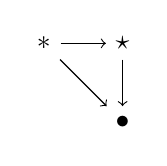
\begin{tikzpicture}
		\node (ast)  {$\ast$};
		\node (star) [right of=ast]{$\star$};
		\node (bull) [below of=star]{$\bullet$};

		\draw[->] (ast) to node {}(star);
		\draw[->] (star)to node {}(bull);
		\draw[->] (ast) to node {}(bull);
	       \end{tikzpicture}
	      \end{center}
	      三つの対象と必要な恒等射,一つめから二つめ,二つめから三つ
	      め,一つめから三つめの対象への射がそれぞれちょうと一つずつ
	      ある(従って最後の射は前二つの射の合成となる).
	\item 圏 {\bf 0}\index{0@{\bf 0}} は次の通り:\\

	      これは対象も射も持たない圏である.
       \end{itemize}
       上のように,以後必要の無い場合は恒等射を省略する.

       有限圏を指定するのは簡単だ------対象を幾つか設定し,公理で要請さ
       れる恒等射を加えて,合成が存在するように対象の間に射を描き入れれ
       ばよい.また,その過程で循環が出来てしまったら,射が有限になるよ
       うに,何らかの等式を置いて取り除かなくてはならない.例えば,次の
       例を考えてみよう:
       \begin{center}
	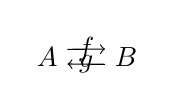
\begin{tikzpicture}
	 \node (A) {$A$};
	 \node (B) [right of=A] {$B$};

	 \draw[->] (A.20) to node {$f$} (B.160);
	 \draw[<-] (A.340) to node [swap]{$g$} (B.200);
	\end{tikzpicture}
       \end{center}
       もし$gf=1_A$などとしてループを取り除かなければ,$gf,
       gfgf,gfgfgf,\ldots$と射の合成が無限に行うことが出来てしまい,圏には
       なるが{\bfseries 有限}圏にはならない.こうした状況については,この章の後半で
       の自由圏について議論する際にまた検討する.
 \item 次の標語は,圏論\index{けんろん@圏論}で重要なスローガンのひとつで
       ある.
       \begin{quote}
	{\bfseries 本当に重要なものは射だけだ!}
       \end{quote}
       という訳で,圏の間の射,或いは「写像\index{しやそう@写像}」を考え
       る必要がある.
       「圏の準同型」\index{けん@圏!のしゆんとうけい@---の準同型}
       \index{しゆんとうけい@準同型!けんの@圏の---}
       は「函手」と呼ばれる.
       \begin{definition}
	圏${\bf C}$と${\bf D}$の間の{\bfseries 函手}
	({\itshape functor})
	\index{かんしゆ@函手|textit}
	\[
	 F : {\bf C} \to {\bf D}
	\]
	とは対象を対象に,射を射に移すマップであって,次を満たすものであ
	る.
	\begin{enumerate}
	 \renewcommand{\labelenumi}{(\alph{enumi})}
	 \item $F(f:A \to B) = F(f) : F(A) \to F(B)$
	 \item $F(1_A) = 1_{F(A)}$
	 \item $F(g \circ f) = F(g) \circ F(f)$
	\end{enumerate}
       \end{definition}
       即ち,$F$は,ドメイン,コドメイン,恒等射と合成を保存するという
       ことである.函手 $F : {\bf C} \to {\bf D}$はしたがって${\bf C}$
       の${\bf D}$の中での(ときたま歪んだ)描像を与える.
       \begin{center}
	\begin{tikzpicture}
	 \matrix (m)[matrix of math nodes,row sep=1.5em,column sep=3em] {
	    & A & B \\
	  {\bf C} \\
	    &   & C \\
	  \\
	    &   & F(B)\\
	  {\bf D} \\
	    & F(A) & F(C) \\
	 };

	 \draw[->] (m-1-2) to node {$f$} (m-1-3);
	 \draw[->] (m-1-3) to node {$g$} (m-3-3);
	 \draw[->] (m-1-2) to node [swap]{$g \circ f$} (m-3-3);

	 \draw[->] (m-2-1) to node [swap]{$F$} (m-6-1);

	 \draw[->] (m-7-2) to node {$F(f)$} (m-5-3);
	 \draw[->] (m-5-3) to node {$F(g)$} (m-7-3);
	 \draw[->] (m-7-2) to node [swap]{$F(g \circ f)$} (m-7-3);
	\end{tikzpicture}
       \end{center}

       さて,期待する通りの方法で函手の合成
       \index{かんしゆ@函手!のこうせい@---の合成}が定義できることも,任意の圏
       ${\bf C}$は恒等函手\index{かんしゆ@函手!こうとう@恒等---}
       $1_{\bf C} : {\bf C} \to {\bf C}$を持つことも
       簡単に判るだろう.こうして我々は新たな圏の例として,全ての圏と函
       手からなる圏,\index{けん@圏!けんの@圏の---} 即ち
       $\Cat$\index{Cat@$\Cat$}を得る.
 \item {\bfseries プレ順序}\index{ふれしゆんしよ@プレ順序|textit}
       ({\itshape preorder};前順序とも\footnote{訳注:「前順序」と「全
       順序」の音が区別できないため,以下では「プレ順序」を用いる.})集
       合とは,反射的かつ推移的な二項関係 $p\leq q$ が入った集合
       $P$のことである.すなわち,$a \leq a$が常に成立し,また
       $a \leq b$かつ$b\leq c$ ならば $a \leq c$が成立しているような集合
       である.任意のプレ順序集合 $P$ は,$P$ の元を対象とし,射を
       \begin{equation}
	a \to b \iff a \leq b \label{preorder}
       \end{equation}
       により一意的に定めてやることで圏と見做すことが出来る.
       \index{けん@圏!ふれしゆんしよ@プレ順序---}
       $\leq$に関する反射律と推移律の条件が $P$ が実際に圏となることを保証している
       のだ.

       逆に,各対象の間に高々一つしか射を持たないような圏は,
       $(\ref{preorder})$ によって対象間に二項関係 $\leq $を定めてやるこ
       とでプレ順序集合と見做すことが出来る.
 \item Poset は自明にプレ順序の条件を満たし,更に反対称律:$a \leq b$ か
       つ $b \leq a$ ならば $a = b$ を満たす.従って特に poset も圏とな
       る.このような{\bfseries poset 圏}\index{けん@圏!poset@poset---}
       は一般的な概念である.例として,任意の集合 $X$ について,冪集合
       $\Pow(X)$は$X$の部分集合$U, V$ の包含関係 $U \subseteq V$
       の下で poset となる.

       Poset 圏 $P, Q$ の間の函手 $F: P \to Q$は何だろうか?
       \index{かんしゆ@函手!posetの@posetの---}
       それは恒等射と合成を保つ写像で……そう,明らかにそれは既に見た単調写像である.
       圏を$p\leq q$以上の構造をもったある種の{\bfseries 一般化された
       poset}であると考えるのはしばしば便利である.したがって,その場合函手は単
       調写像の一般化と見做すことが出来る.
 \item {\bfseries 位相空間の例:}$X$ を位相空間,${\cal O}(X)$をその開集
       合系とすると,${\cal O}(X)$ は包含関係について poset 圏になる.更
       に,任意の開集合$U$に対して$x\leq y\ \text{iff}\ x \in U\
       \text{ならば}\ y \in U$ によって $X$ の各点 $x,y \in X$について
       {\bfseries 特殊化}順序
       \index{いそうのとくしゆかしゆんしよ@位相の特殊化順序}
       を入れることで,X はプレ順序集合となる.
       つまり,開集合 $U$ が$x$を含めば必ず $y$ も含むとき, $x \leq y$
       とするのである.もし$X$が十分に分離されていれば(「$T_1$」空間な
       ら)順序は自明なものになってしまうが,そうでない場合が非常に興味
       深いものとなる.そうした例は例えば代数幾何や表示的意味論
       \index{ひようしてきいみろん@表示的意味論}の理論で出て
       来る.$T_0$ 空間がこの特殊化順序の下で実際に poset となることは演
       習問題とする.
 \item {\bfseries 論理学の例:}\index{ろんりかく@論理学}
       ある論理の推論系が与えられた時,関連する
       {\bfseries 証明の圏}\index{けん@圏!しようめいの@証明の---}が存在する.
       証明の圏の対象は論理式:
       \[
	\phi, \psi,\ldots
       \]
       であり,$\phi$ から $\psi$ への射は,$\phi$ を仮定して $\psi$ を
       演繹\index{えんえき@演繹}する証明木:
       \label{example of logic}
	\begin{center}
	 \AxiomC{$\phi$}
	 \UnaryInfC{$\vdots$}
	 \UnaryInfC{$\psi$}
	 \DisplayProof
	\end{center}
       である(但し仮定$\phi$は推論の途中でキャンセルされないものとする).
       射の合成は演繹の自明な合成で与えられ,これは明らかに結合的である
       (恒等射$1_\phi$は何か?).証明の過程によって,
       \[
	p: \phi \to \psi
       \]
       は複数存在しうることに注意したい.この圏はとても豊かな構造を持っ
       ており,後ほど$\lambda$計算\index{らむたけいさん@ラムダ計算}
       \index{らむたけいさん@$\lambda$計算|see{ラムダ計算}}
       と関連して再び取り上げる.
 \item {\bfseries 計算機科学の例:}\index{けいさんきかかく@計算機科学}
       関数型プログラミング言語
       \index{ふろくらみんくけんこ@プログラミング言語}$L$が与えられ
       たとき,対象を $L$のデータ型\index{てーたかた@データ型},
       射を$L$の計算可能函数(「プロセス」,「手続き」,「プログラム」)
       とする圏を考えることが出来る.
       そうした二つのプログラム$X\xrightarrow{f} Y \xrightarrow{g} Z$の
       合成は,$f$の出力に$g$を適用することで与えられ,
       \[
	g \circ f = f;g
       \]
       などと書かれたりする.恒等射は「何もしない」プログラムである.

       このような圏はプログラミング言語の表示的意味論の分野で基本的な考
       え方である.例えば,いま上で定義した圏を${\bf C}(L)$とすると,
       プログラミング言語 $L$ の Scott 領域${\bf D}$における表示的意
       味論とは,単に函手
       \[
	S: {\bf C}(L) \to {\bf D}
       \]
       のことである.ここで$S$は型に領域を,プログラムに連続写像を割り当
       てる函手である.この例と先程の例は,共に後で考察する「デカルト閉
       圏」
       \index{けん@圏!てかるとへい@デカルト閉---}の概念と関係がある.
 \item $X$を集合とする.$X$の元を対象,射をそれらの恒等射のみとすること
       で,$X$を圏${\bf Dis}(X)$と見做すことが出来る.このように射が恒等
       射だけである圏は{\bfseries 離散圏}
       \index{けん@圏!りさん@離散---|textit}と呼ばれる.離散圏は単に poset
       の特別な場合に過ぎないことに注意したい.
 \item {\bfseries モノイド}\index{ものいと@モノイド|textit}
       ({\bfseries 単位的半群\index{はんくん@半群}}とも呼ばれる)とは,
       二項演算子$\cdot:M\times M \to M$ と特別な「単位元」$u\in M$を持
       つ集合 $M$ であって,任意の$x,y,z \in M$について,
       \[
	x \cdot (y \cdot z) = (x \cdot y) \cdot z
       \]
       かつ
       \[
	u \cdot x = x = x \cdot u
       \]
       を満たすものである.モノイドは対象がただ一つである圏と等価である.
       \index{けん@圏!ものいと@モノイド---}
       圏の射に当るものが$M$の元であり,特に恒等射に対応するものが単位元
       $u$である.射の合成はモノイドの二項演算$m \cdot n$で与えられる.

       モノイドはとても一般的な構造である.たとえば,$\N, \Q, \R$ と,加
       法と$0$についてのモノイドや,同じく乗法と $1$についてのモノイドな
       ど,数\index{すう@数}からなるモノイドがある.
       それ以外にも,任意の集\index{しゆうこう@集合}合$X$について,$X$か
       ら$X$への写像全体の集合
       \[
	\Hom_{\Sets}(X,X)
       \]
       \index{Homしゆうごう@Hom集合}
       も合成についてモノイドを成す.更に一般に,圏${\bf C}$についてその
       対象$C$上の射全体
       \[
	\Hom_{\bf C}(C, C)
       \]
       も射の合成についてモノイドになる.

       モノイドは構造の入った集合
       \index{しゆうこう@集合!こうそうのはいつた@構造の入った---}なの
       で,モノイドを対象,モノイド構造を保存する写像を射とした圏
       $\Mon$\index{Mon@$\Mon$}がある.詳しくいえば,モノイド$M$から$N$
       への準同型 \index{しゆんとうけい@準同型!ものいと@モノイド---}
       とは,写像$h: M \to N$であって,任意の$m, n \in M$ に対して,
       \[
	h(m \cdot_M n) = h(m) \cdot_N h(n)
       \]
       と
       \[
	h(u_M) = u_N
       \]
       を満たす物である.モノイド準同型$f: M \to N$は,$M, N$を圏と見做
       したときの函手と同じものであることに注意したい.この意味で,圏は
       モノイドの,函手は準同型の一般化になっている.
\end{enumerate}
\section{同型射}
\begin{definition}
 任意の圏${\bf C}$について,射$f: A \to B $が{\bfseries 同型射}
 ({\itshape isomorphism})
 % \index{とうけいしや@同型射|textit}
 であるとは,ある${\bf C}$の射$g: B \to A$が存在して,
 \[
  g \circ f = 1_A\ \ \text{かつ}\ \ f \circ g = 1_B
 \]
 が成り立つことである.逆射は一意なので(証明せよ!),$g = f^{-1}$と書く.
 $A$ と $B$の間に同型射が存在するとき,$A$ は $B$ と{\bfseries 同型}
 \index{とうけい@同型|textit}
 ({\itshape isomorphic})であるといわれ,$A \cong B$ と書く.
\end{definition}
\index{とうけいしや@同型射|(}
この同型射の定義が,重要な概念の{\bfseries 抽象的}・圏論
\index{けんろん@圏論}的な定義として採り上げる最初の例である.
純粋に圏論的な概念だけを使い,射や対象についての他の追加的な情報
を一切使っていないという意味において,これは抽象的な定義である.
こうすることで,他のどんな圏であっても同じ定義を使うことが出来るという利
点がある.例えば,集合(またはモノイド)としての同型を,
{\bfseries 全単射},つまり「1対1かつ上への」写像
\index{しやそう@写像!せんたんしや@全単射---}(または準同型)として元
に言及する形で定義することがある.集合やモノイドなどの場合,こうした定義
は我々の圏論を用いた定義と同値である.一方,注意すべきなのは,例えば
$\Pos$では上の圏論的な同型の定義はうまくゆくのに対し,「全単射な準同型」
が存在するにもかかわらず同型でないような Poset が存在する.更にいえば,
モノイドを圏と見做した場合のように,抽象的な定義{\bfseries のみ}がきちん
とした意味を持つような例は沢山ある.

\begin{definition}
 群$G$\index{くん@群|textit}とは,任意の元$g$に対してその逆元$g^{-1}$が
 存在しているモノイドである.従って,$G$はただ一つの対象を持ち,全ての射
 が同型射であるような圏である.
\end{definition}

自然数の全体$\N$は加法についても乗法についても群にならないが,$\Z$は加法
について,$\Q$は乗法についてそれぞれ群を成す.\index{すう@数}任意の集合
 $X$ について,その自己同型\index{しことうけい@自己同型}(或いは「置
 換」),即ち同型射 $f: X \to X$ からなる群$Aut(X)$がある(合成「$\circ$」
 について閉じているのは何故か?).集合$X$の{\bfseries 置換群}
 \index{くん@群!ちかん@置換---}({\itshape group of permitations})とは,
 部分集合$G \subseteq Aut(X)$ であっ
 て,$X$ の自己同型(のうちの幾つか)から成る群である.従って,$G$は次の
 条件を満たさなくてはらなない:
\begin{enumerate}
 \item $X$上の恒等写像 $1_X$ を元に持つ
 \item $g, g' \in G$ ならば $g \circ g' \in G$
 \item $g \in G$ ならば $g^{-1} \in G$
\end{enumerate}

群の準同型$h:G \to H$は単にモノイドとしての準同型であり,必然的に逆元も
保存される(証明せよ).\index{しゆんとうけい@準同型!くん@群---}

さて,抽象群に関する次の基礎的かつ古典的な定理について考えよう.

\index{Cayleyのていり@Cayleyの定理|(}
\begin{theorem*}[Cayley]
 任意の群 $G$ はある置換群と同型である.
\end{theorem*}
\begin{proof}[証明 \textup({\bfseries 概略}\textup)]
  
 \begin{enumerate}
  \item まず,$G$の Cayley 表現\index{ひようけん@表現} $\bar G$を次の集
	合の置換群として定義する:
	集合は$G$自身とし,任意の元$g \in G$に対して置換$\bar g :  G \to G$
	を,任意の$h\in G$に対して「左平行移動」
	\[
	\bar g(h) = g \cdot h
	\]
	で定義する.$\bar{g^{-1}}$が$\bar g$の逆写像になっているので,これは実
	際に順列となる.
  \item 次に準同型 $i: G \to \bar G$ を $i(g) = \bar g$ で,$j: \bar G
	\to G$ を $j(\bar g) = g(u)$ で定義する.
  \item 最後に $i \circ j = 1_{\bar G}$ と $j \circ i = 1_G$ を示す.
 \end{enumerate}
\end{proof}
\begin{warn}
 Cayleyの定理の証明には異なる二つのレベルの同型射が現れていることに注意せ
 よ.まず$\Sets$の同型射としての$G$の順列があり,群と群準同型のなす圏
 ${\bf Groups}$での同型射が $G$ と $\bar G$の間に存在するのである.
\end{warn}
Cayley の定理の主張は,どんな抽象的な群も,ある集合の置換群として「具体
的」に表現出来るということである.この定理は,「大きすぎない」任意の圏
\index{けん@圏!ちいさな@小さな---}が「具体圏」としての表現を持つ,という
形で一般化することが出来る(圏が「大きすぎ」ないことの技術的な定義は
\ref{sec:foundations}節で詳しく見る).

\begin{theorem}
 射の集合を持つ任意の圏${\bf C}$は,集合を対象,その間の写像を射とする圏と同型
 である.
\end{theorem}
\begin{proof}[証明 \textup({\bfseries 概略}\textup)]
 圏${\bf C}$の Cayley 表現$\bar{\bf C}$を次の具体圏として定義する:
 \begin{itemize}
  \item 対象は,任意の $C \in {\bf C}$に対し
	\[
	 \bar C = \set{ f \in C | \cod(f) = C}
	\]
	の形の集合.
  \item ${\bf C}$の射 $g: C \to D$ に対応する射
	\[
	 g: \bar C \to \bar D
	\]
	は,任意の$\bar{\bf C}$の対象$f: X \to C$に対し $\bar g(f) = g
	\circ f$ で定義される写像.
	\begin{center}
	 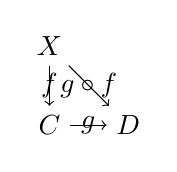
\begin{tikzpicture}
	 \node (X) {$X$};
	 \node (C) [below of=X]{$C$};
	 \node (D) [right of=C]{$D$};

	 \draw[->] (X) to node [swap]{$f$} (C);
	 \draw[->] (X) to node {$g \circ f$} (D);
	 \draw[->] (C) to node [swap] {$g$} (D);
	\end{tikzpicture}\end{center}
 \end{itemize}
\end{proof}
\index{Cayleyのていり@Cayleyの定理|)}
\begin{remark}
 この例は,集合圏における「具体」圏\index{けん@圏!くたい@具体---}につい
 ての素朴な見方の {\bfseries 誤り}を教えてくれる.つまり,全ての圏がある
 種の函数や集合を射や対象として持つとは限らないが,どのような圏もそんな圏
 と同型なのである.従って,そうした圏だけが満たすような性質は圏論的には
 全く関係のないものに限られ,例えば射に影響しないような対象の特徴は捨て
 去られる(これは,実数の構成法に Dedekind 切断を用いるのか Cauchy列を用
 いるのかの違いと似たようなものである).「具体」圏の概念を理解するのに
 幾分ましな解釈は,どんな射$f:C\to D$も任意の「試験対象」$T$
 \index{しけんたいしよう@試験対象}
 からの射$x: T\to C$との合成によって決定される,という考え方である.ここ
 で「決定される」というのはそのような任意の $x$ に対して $fx = gx$ な
 らば $f = g$が 成立する,という意味である.これは,$T$による圏の表現を
 考察していること と同じである. この条件が
 第\ref{Ch:initial and terminal objects}節で定義される「終対象」
 $T$について成立 しているとき,その圏は「具体圏」であるとされる.一方,
 第\ref{Ch:Abstract Structure}章で見るように, $T$として終対象以外の対象
 を取ったほうが良い場合もある.

 圏${\bf C}$が「射の集合をもつ」という条件が
 $\set{f \in {\bf C} | \cod(f) = C}$ が実際に集合\index{しゆうこう@集合}
 になることを保証していることに注意したい. 第\ref{sec:foundations}節で
 この点について立ち返る.
\end{remark}
\index{とうけいしや@同型射|)}

\section{圏の構築}
\index{けん@圏!のこうちく@---の構築|(}
考察の対象となる圏のストックが沢山あるので,今度は既にある圏から新た
な圏を構成する方法について考えることが出来る.

\begin{enumerate}
 \item 二つの圏${\bf C}, {\bf D}$の{\bfseries 直積}
       \[
	{\bf C} \times {\bf D}
       \]
       は,対象$C \in {\bf C}, D \in {\bf D}$ について$(C, D)$の形を対象
       として持ち,射は $f: C \to C' \in {\bf C}, g: D \to D' \in {\bf
       D}$ に対して
       \[
	(f, g) : (C, D) \to (C', D')
       \]
       の形のものである.合成と恒等射は要素ごとに定義される.即ち:
       \begin{align*}
	(f', g') \circ (f, g) &= (f' \circ f, g \circ g)\\
	            1_{(C,D)} &= (1_C, 1_D)
       \end{align*}
       圏の直積に対し,二つの自明な{\bfseries 射影函手}
       \index{かんしゆ@函手!しやえい@射影---}
       \begin{center}
	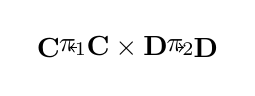
\begin{tikzpicture}
	 \node (CD) {${\bf C} \times {\bf D}$};
	 \node (C) [left of=CD] {${\bf C}$};
	 \node (D) [right of=CD]{${\bf D}$};

	 \draw[->] (CD) to node [swap]{$\pi_1$} (C);
	 \draw[->] (CD) to node {$\pi_2$} (D);
	\end{tikzpicture}
       \end{center}
       がある.$\pi_1(C,D) = C$ かつ $\pi_1(f,g) = f$ で定義
       され,$\pi_2$ も同様である.

       群\index{くん@群}に慣れていれば,群 $G, H$ を圏と見做したときの直
       積圏$G \times H$ \index{けん@圏!ちよくせき@直積---|textit}
       が通常の群としての直積と一致することに気が付くだろう.
 \item 圏${\bf C}$ の{\bfseries 逆圏}\index{けん@圏!きやく@逆---|textit}
       ({\itshape opposite category})
       (または「双対圏」\index{けん@圏!そうつい@双対---}({\itshape dual
       category}))
       ${\bf C}^{\rm op}$は${\bf C}$と同じ対象を持ち,${\bf C}^{\rm op}$
       の射 $f: C \to D$ は ${\bf C}$ の射 $f: C \to D$ である.
       つまり,${\bf C}^{\rm op}$ とは,${\bf C}$の射の向きを全てひっく
       り返した圏である.

       ${\bf C}$と ${\bf C}^{\rm op}$の対象・射を区別する記法があった方
       が便利なので,${\bf C}$ の射 $f: C \to D$ に対応する ${\bf
       C}^{\rm op }$の射を,
       \[
	f^*: D^* \to C^*
       \]
       と書くことにする.この記法の下で,${\bf C}$ の対応する操作を用い
       て${\bf C}^{\rm op}$での合成と恒等射を次で定義することが出来る.
       \begin{align*}
	1_{C^*}       &= (1_C)^*\\
	f^* \circ g^* &= (g \circ f)^*
       \end{align*}

       従って,${\bf C}$ での図式
       \begin{center}
	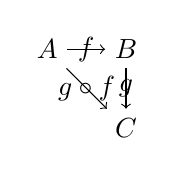
\begin{tikzpicture}
	 \node (A) {$A$};
	 \node (B) [right of=A] {$B$};
	 \node (C) [below of=B] {$C$};

	 \draw[->] (A) to node {$f$} (B);
	 \draw[->] (B) to node {$g$} (C);
	 \draw[->] (A) to node [swap] {$g \circ f$} (C);
	\end{tikzpicture}
       \end{center}
       は ${\bf C}^{\rm op}$ 内では次のようになる.
       \begin{center}
	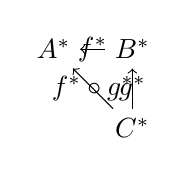
\begin{tikzpicture}
	 \node (A) {$A^*$};
	 \node (B) [right of=A] {$B^*$};
	 \node (C) [below of=B] {$C^*$};

	 \draw[<-] (A) to node {$f^*$} (B);
	 \draw[<-] (B) to node {$g^*$} (C);
	 \draw[<-] (A) to node [swap] {$f^* \circ g^*$} (C);
	\end{tikzpicture}
       \end{center}
       数学の「双対性」\index{そうついせい@双対性}に関する定理の多くは,
       ある圏がある圏の双対圏(の部分圏)であるという事実を表現したもの
       である.その種の例としては,後で扱う$\Sets$ が完備原子的ブール代数
       \index{ふーるたいすう@ブール代数}の圏の双対である,というようなものがある.
       
 \item 圏${\bf C}$の{\bfseries 射圏}\index{けん@圏!しや@射---|textit}
       ({\itshape arrow category})
       ${\bf C}^{\to}$ とは,${\bf C}$の射を対
       象とし,$f: A \to B$ から $f': A' \to B'$ への射 $g$ は,次の「可
       換四角形」である.
       \begin{center}
	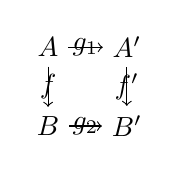
\begin{tikzpicture}
	 \node (A) {$A$};
	 \node (A') [right of=A] {$A'$};
	 \node (B)  [below of=A] {$B$};
	 \node (B') [right of=B] {$B'$};

	 \draw[->] (A)  to node {$g_1$} (A');
	 \draw[->] (A)  to node [swap]{$f$}   (B);
	 \draw[->] (A') to node {$f'$}  (B');
	 \draw[->] (B)  to node [swap]{$g_2$} (B');
	\end{tikzpicture}
       \end{center}
       ここで,$g_1, g_2$ は ${\bf C}$ の射.つまり,${\bf C}^{\to}$の射は
       次を満たすような射 $g_1, g_2$ の対 $(g_1, g_2)$ である.
       \[
	g_2 \circ f = f' \circ g_1
       \]
       対象$f : A \to B$ 上の恒等射$1_f$ は対 $(1_A, 1_B)$で,射の合成は
       要素ごとに行えばよい.
       \[
	(h_1, h_2) \circ (g_1, g_2) = (h_1 \circ g_1, h_2 \circ g_2)
       \]

       読者はこの定義で上手くゆくことを,可換図式を書いて確認せよ.

       以下の二つの函手があることも確認せよ.
       \begin{center}
	
\begin{tikzpicture}
	 \node (C1) {${\bf C}$};
	 \node (C->) [right of=C1] {${\bf C}^{\to}$};
	 \node (C2)  [right of=C->] {${\bf C}$};

	 \draw[<-] (C1) to node {${\bf dom}$} (C->);
	 \draw[->] (C->) to node {${\bf cod}$} (C2);
	\end{tikzpicture}
       \end{center}
 \item 圏 ${\bf C}$の対象$C \in {\bf C}$ 上の{\bfseries スライス圏}${\bf C}/C$
       \index{けん@圏!すらいす@スライス---|textit}とは,以下の対象・射を持つ圏である.
       \begin{itemize}
	\item 対象:$\cod(f) = C$ なる任意の射 $f \in {\bf C}$
	\item 射:$f: X \to C$ から $f': X' \to C$ への射は,下の図式で
	      表されるような$f' \circ a = f$ を満たす ${\bf C}$ の射 $a :
	      X \to X'$.
	      \begin{center}
	       \begin{tikzpicture}
		\node (X)  at (0,2) {$X$};
		\node (X') at (4,2) {$X'$};
		\node (C)  at (2,0) {$C$};

		\draw[->] (X) to node {$a$} (X');
		\draw[->] (X) to node [swap]{$f$} (C);
		\draw[->] (X') to node {$f'$} (C);
	       \end{tikzpicture}
	      \end{center}
       \end{itemize}
       恒等射と合成については,射圏と同様に ${\bf C}$ のものを流用する.
       「基底対象 $C$ を忘れる」函手 $U: {\bf C}/ C \to {\bf C}$ が存在する
       ことを注意しておく.

       $g: C \to D$ を ${\bf C}$ の任意の射としたとき,$g_*(f) = g \circ
       f$ で定義される合成函手
       \[
	g_*: {\bf C}/C \to {\bf C}/D
       \]
       が存在して,
       \begin{center}
	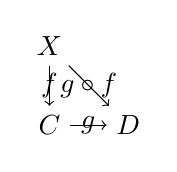
\begin{tikzpicture}
	 \node (X) {$X$};
	 \node (C) [below of=X] {$C$};
	 \node (D) [right of=C] {$D$};

	 \draw[->] (X) to node {$g \circ f$} (D);
	 \draw[->] (X) to node [swap]{$f$} (C);
	 \draw[->] (C) to node [swap]{$g$} (D);
	\end{tikzpicture}
       \end{center}
       ${\bf C}/C$ の射についても同様に定義されているものとする.実際,簡
       単に確認出来るように,スライス圏の構成法自体が函手
       \[
	{\bf C/(-)} : {\bf C} \to \Cat
       \]
       になっている.Cayley 表現が集合と写像の圏による${\bf C}$の表現を与
       えているのに対して,この函手は圏と函手からなる圏として${\bf C}$の表
       現を与えている.勿論,Cayley 表現とは,圏をその対象の集合に移す忘
       却函手\index{かんしゆ@函手!ほうきやく@忘却---}
       $U: \Cat \to \Sets$ を ${\bf C}/(-)$ の後に合成したものに過ぎない.

       もし,${\bf C} = {\bf P}$ が poset圏\index{けん@圏!poset@poset---}
       で $p \in {\bf P}$ ならば,
       \[
	{\bf P}/p \cong\, \downarrow(p)
       \]
       となる.つまり,スライス圏${\bf P}/p$は,$q \leq p$ なる
       任意の $q \in {\bf P}$ からなる単項イデアル $\downarrow(p)$となる.
       \index{いてある@イデアル}
       他のスライス圏の例はすぐ後で見ることになる.

       圏 ${\bf C}$ の対象 $C$下の{\bfseries コスライス圏}
       \index{けん@圏!こすらいす@コスライス---|textit} $C/{\bf C}$は,
       対象として $\dom(f) = C$ なる任意の${\bf C}$の射$f$を,$f: C \to
       X$ から $f': C \to X'$ への射として $h \circ f = f'$ なる射 $h: X
       \to X'$ を持つ圏である.読者は残りの定義をスライス圏からの類推で
       考えるべきである.また,コスライス圏をスライス圏と双対圏の言葉で
       定義するにはどうすればいいだろうか?
\end{enumerate}
\begin{example}
 {\bfseries 基点つき集合}({\itshape pointed set})の圏
 \index{しゆうこう@集合!きてんつき@基点つき---}
 \index{けん@圏!きてんつきしゆうこうの@基点つき集合の---}
 $\Sets_*$ \index{Sets*@$\Sets_*$}は,集合 $A$ とある点 $a\in A$の
 組を対象とし,射 $f: (A, a) \to (B, b)$ を「基点を保つ」,つまり
 $f(a) = b$ を満たす写像 $f: A \to B$ とする圏である.これは,$\Sets$ 
 の一点集合 $1 = \{*\}$下のコスライス圏と同型である.
 \[
  \Sets_* \cong 1/\Sets
 \]
 実際,写像 $a: 1 \to A$は,$A$の元 と$a(*) = a \in A$ という形で一意に
 対応し,射$f: (A, a) \to (B, b)$ は可換三角形と厳密に対応する.
 \begin{center}
  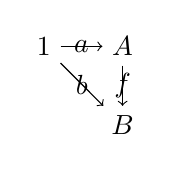
\begin{tikzpicture}
   \node (1) {$1$};
   \node (A) [right of=1] {$A$};
   \node (B) [below of=A] {$B$};

   \draw[->] (1) to node {$a$} (A);
   \draw[->] (1) to node [swap]{$b$} (B);
   \draw[->] (A) to node {$f$} (B);
  \end{tikzpicture}
 \end{center}
\end{example}
\index{けん@圏!のこうちく@---の構築|)}
\section{自由圏}
\label{sec:free categories}
\index{けん@圏!しゆう@自由---|(}
\subparagraph{自由モノイド.}
\index{ものいと@モノイド!しゆう@自由---|(}
% \begin{freemonoid}
 「文字」a, b, c,\ldots の「アルファベット」 $A$,
 つまり集合
 \[
 A = \{a, b, c,\ldots\}
 \]
 から始めよう.$A$上の{\bfseries 語}\index{こ@語}とは,次のような文字の有限列である.
 \begin{center}
 {\itshape thisword}, {\itshape categoriesarefun}, {\itshape asddjbnzzfj},\ldots
 \end{center}
 空の語\index{こ@語!からの@空の---}を表すのに``$-$''と書くことにする.$A$の「Kleene閉包
 \index{Kleeneへいほう@Kleene閉包}」とは次で定義される集合のことである.
 \[
 A^* = \{A\text{上の語}\}
 \]
 $A^*$上の二項演算子$*$を,任意の語$w, w' \in A^*$ に対して $w * w' =
 ww'$で定義する.即ち,$*$ は{\bfseries 連結(連接)}
 \index{れんけつ@連結}\index{れんせつ@連接|see{連結}}操作である.この時演
 算``$*$''は結合的であり,空語 ``$-$'' が単位元となるので,$A^*$はモノイドと
 なる.特に,$A^*$ は $A$上の{\bfseries 自由モノイド}
 \index{しゆう@自由!ものいと@---モノイド}
 と呼ばれる.任意の元
 $a \in A$は長さ 1 の語と見做せることから,$i(a) = a$ で定義され,「生成
 元の埋め込み」
 \index{せいせいけん@生成元}
 \index{せいせいけん@生成元!のうめこみ@---の埋め込み}
 と呼ばれる写像
 \[
 i: A \to A^\ast
 \]
 を得る.どんな$w \in A^\ast$も,ある$a_1, a_2,\ldots,a_n$の$*$-積として $w
 = a_1 * a_2 * \ldots * a_n$と表せるという意味において,$A$の元は自由モノ
 イドを「生成する」という.
% \end{freemonoid}

さて,ここでいう「自由」\index{しゆう@自由}とはどういう意味だろうか?
「代数の初歩」のような本で,次のような記述を読んだことがある読者もいるかもしれない:

モノイド$M$が次の条件を満たす時,$M$は$M$の部分集合$A$によって{\bfseries
自由に生成される}({\itshape freely generated} by $A$)という.
\begin{enumerate}
 \item 任意の元 $m \in M$ は$A$の元の積として表せる.即ち:
       \[
	m = a_1 \cdot_M \ldots \cdot_M a_n,\ \ \ a\_i \in A
       \]
 \item $M$に「非自明な」関係が存在しない.つまり,$a_1 \ldots a_j = a'_1
       \ldots a'_k$なる等式が成立するならば,それはモノイドの公理から証明
       できなくてはならない.
\end{enumerate}
最初の条件は「ゴミ\index{こみ@ゴミ}なし」,二つめの条件は
「ノイズ\index{のいす@ノイズ}なし」と時々呼ばれたりす
る.つまり,$A$上の自由モノイドとは,$A$を含みゴミもノイズも持たないモノ
イド,ということになる.この自由モノイドの定義をどう思うだろうか?

筆者としては,二番目の条件の中の「証明可能性」といった表現に異を唱えたい.
もっと定義として精確な表現が存在する筈だ.圏論を用いれば,
定義の意味を汲みつつ,より曖昧性のない精確な「自由」の定義を与えることが
できる.

まず,どんなモノイド$N$に対してもその台集合$|N|$があり,またモノイド準
同型$f: M \to N$ に対しても台写像 $|f| : |M| \to |N|$ を考えることが出来
る.この対応が函手を与えることは簡単に確認できる.このような函手を「忘却
函手(forgetful functor)」\index{かんしゆ@函手!ほうきやく@忘却---}
という.すると,集合$A$上の自由モノイド$M(A)$は,
次の{\bfseries 普遍写像性}({\itshape universal mapping property}, UMP)
\index{ふへん@普遍}\index{ふへんしやそうせい@普遍写像性}
\index{UMP|see{普遍写像性}}
を満たすモノイドとして定義することが出来る!

\begin{UMPofFreeMonoid}
 % \index{ものいと@モノイド!しゆう@自由---|textit}
 \index{ふへんしやそうせい@普遍写像性!しゆうものいとの@自由モノイドの---|textit}
 写像$i: A \to |M(A)|$があり,任意のモノイド$N$と写像$f: A \to |N|$が与え
 られたとき,$|\bar f|\circ i = f$を満たすようなモノイド準同型 $\bar f:
 M(A) \to N$ が一意に存在する.つまり,次の可換図式が成立する.

 $\Mon$において:
 \begin{center}
 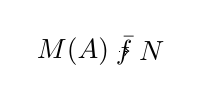
\begin{tikzpicture}
  \node (MA) {$M(A)$};
  \node (N) [right of=MA] {$N$};
  \draw[->, dotted] (MA) to node {$\bar f$} (N);
 \end{tikzpicture}
 \end{center}

 $\Sets$において:
 \begin{center}
 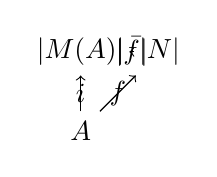
\begin{tikzpicture}
  \node (MA) {$|M(A)|$};
  \node (N) [right of=MA] {$|N|$};
  \node (A) [below of=MA] {$A$};
  \draw[->] (MA) to node {$|\bar f|$} (N);
  \draw[->] (A) to node {$i$} (MA);
  \draw[->] (A) to node [swap]{$f$} (N);
 \end{tikzpicture}
 \end{center}
\end{UMPofFreeMonoid}
\begin{prop}
 $A^*$ は $A$ 上の自由モノイドの普遍写像性を持つ.
\end{prop}
\begin{proof}[証明]
 $f:A \to |N|$ が与えられたとき,次の式で $\bar f: A^\ast \to N$ を定義
 する.
 \begin{align*}
  \bar f(-) &= u_N,\ \ \ \text{$N$の単位元}\\
  \bar f(a_1 \ldots a_i) &= f(a_1) \cdot_N \ldots \cdot_N f(a_i)
 \end{align*}
 このとき,$\bar f$ は明らかに準同型であり,任意の $a\in A$に対し
 \[
  \bar f(a) = f(a)
 \]
 を満たす.また,$g: A^\ast \to N$ が任意の$a\in A$に対して$g(a) = f(a)$
 を満たせば任意の $a_1\ldots a_i \in A$ に対し:
 \begin{align*}
  g(a_1 \ldots a_i) &= g(a_1 * \ldots * a_i)\\
                    &= g(a_1) \cdot_N \ldots \cdot_N g(a_i)\\
                    &= f(a_1) \cdot_N \ldots \cdot_N f(a_i)\\
                    &= \bar f(a_1) \cdot_N \ldots \cdot_N \bar f(a_i)\\
                    &= \bar f(a_1 * \ldots * a_i)\\
                    &= \bar f(a_1 \dots a_i)
 \end{align*}
 よって$g = \bar f$となる.
\end{proof}
なぜ上の普遍写像性が自由モノイドの「ゴミなし」「ノイズなし」の意味を精確に表
現出来ているのかについて考えよう.特に,普遍写像性の「存在」の部分が「ノイズ
\index{のいす@ノイズ}なし」の曖昧な意図を捉えたものであり(生成元の代数
的な組合せによる等式は,どんな写像の行き先でも,つまりどこでも成立しなく
てはならないから),「一意性」の部分が「ゴミ\index{こみ@ゴミ}なし」のア
イデアを精確化している(生成元の組合せによって表現されない余分な元がある
と,写像によって行き先が{\bfseries 異なる}可能性があり,一意性が破れてし
まう).

以上の普遍写像性を用いれば,$A$上の自由モノイドが次の意味で同型を除いて一意で
あることが示すことが出来る.

\begin{prop}
 モノイド$M, N$と写像 $i: A \to |M|,\, j: A \to |N|$ が与えられ,それぞ
 れ$A$上の自由モノイドの普遍写像性を満たすとき,$|h|i = j$ かつ
 $|h^{-1}|j=i$ を満たすモノイド同型 \index{とうけいしや@同型射}
 $h: M \cong N$が一意に存在する.
\end{prop}
\begin{proof}[証明]
 $M$ の普遍写像性と $j$ から $|\bar j|i = j$ を満たす $\bar j: M \to N$が,
 $N$の普遍写像性と $i$ から $|\bar i|j = i$ を満たす $\bar i: N \to M$ がそ
 れぞれ一意に存在する.その合成は準同型 $\bar i \circ \bar j: M \to M$
 であり,$|\bar i \circ \bar j|i = i$を満たす.今,特に $1_M: M \to M$
 もこの性質\index{しやそう@写像!のせいしつ@---の性質|see{普遍写像性}}
 を満たすので,$M$の普遍写像性の一意性より$\bar i \circ \bar j =
 1_M$ がいえる.$M$ と $N$ の役割を交換すれば同様にして $\bar j \circ
 \bar i = 1_N$ を得る.

 $\Mon$において:
 \begin{center}
  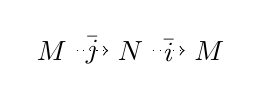
\begin{tikzpicture}
   \node (M1) {$M$};
   \node (N) [right of=M1] {$N$};
   \node (M2) [right of=N] {$M$};

   \draw[->, dotted] (M1) to node {$\bar j$} (N);
   \draw[->, dotted] (N) to node {$\bar i$} (M2);
  \end{tikzpicture}
 \end{center}

 $\Sets$において:
 \begin{center}
  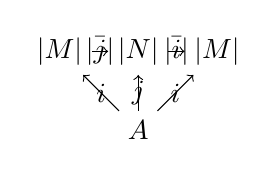
\begin{tikzpicture}
   \node (M1) {$|M|$};
   \node (N) [right of=M1] {$|N|$};
   \node (M2) [right of=N] {$|M|$};
   \node (A) [below of=N] {$A$};

   \draw[->] (M1) to node {$|\bar j|$} (N);
   \draw[->] (N) to node {$|\bar i|$} (M2);
   \draw[->] (A) to node {$i$} (M1);
   \draw[->] (A) to node [swap]{$i$} (M2);
   \draw[->] (A) to node {$j$} (N);
  \end{tikzpicture}
 \end{center}
\end{proof}

たとえば,一点集合上の任意のモノイドは$\N$の加法についての\index{すう@数}数
モノイド(「生成元」は1)と同型であることが容易にわかる.従って,モノイドとしての$\N$
は,自由モノイドの普遍写像性により同型を除いて一意に決定される.
\index{ものいと@モノイド!しゆう@自由---|)}

\subparagraph{自由圏.}
\index{しゆう@自由!けん@---圏}
今やったことを,モノイドだけではなく圏にも一般化しよ
う.圏には台集合のかわりに台グラフがあるので,まずはそこから見ていこう.

{\bfseries 有向グラフ}\index{くらふ@グラフ!ゆうこう@有向---|textit}
({\itshape directed graph})
は頂点と向きを持った辺から成る.即ち各辺には
始点(source)と終点(target)と呼ばれる頂点が与えられている.
\begin{center}
 \begin{tikzpicture}
  \matrix (m) [matrix of math nodes,row sep=2cm,column sep=2cm] {
  A & B\\
  C & D\\
  };
  \draw[->] (m-1-1) to node {$z$}(m-1-2);
  \draw[->] (m-1-1) to node [swap]{$u$}(m-2-2);
  \draw[->] (m-2-1) to node {$x$}(m-1-1);
  \draw[->] (m-2-2) to node [swap]{$y$}(m-1-2);
 \end{tikzpicture}
\end{center}
グラフは圏と同じような図式で描くことが出来るが,辺の合成や恒等射に当るよ
うなものは存在しない.

したがって,グラフは二つの集合 $E$(Edges, 辺)と $V$(Vetrices, 頂点)およ
び二つの写像$s: E \to V$(source, 始点)と$t: E \to V$(target, 終点)か
らなる.よって,$\Sets$においてグラフとは次の形をした対象と射をもつ構造
物である.
\begin{center}
 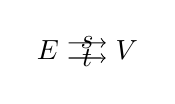
\begin{tikzpicture}
  \node (E) {$E$};
  \node (V) [right of=E]{$V$};

  \draw[->] (E.20) to node {$s$} (V.160);
  \draw[->] (E.340) to node [swap]{$t$} (V.200);
 \end{tikzpicture}
\end{center}

さて,どんなグラフ$G$も,$G$上の自由圏 ${\bf C}(G)$を生成する.${\bf
C}(G)$は $G$ の頂点を対象に,$G$の{\bfseries 道}({\itshape path})を射
に持つ圏である.ここで道とは,辺$e_1,\ldots,e_n$の有限列であって,任意の
$i = 1,\ldots,n$について $t(e_i) = s(e_{i+1})$を満たすものである.
\begin{center}
 \begin{tikzpicture}
  \matrix (m) [matrix of math nodes, row sep=1.5cm, column sep=1.5cm] {
  v_0 & v_1 & v_2 & \dots & v_n\\
  };
  \draw[->]
    (m-1-1) edge node[auto] {$e_1$} (m-1-2) 
    (m-1-2) edge node[auto] {$e_2$} (m-1-3)
    (m-1-3) edge node[auto] {$e_3$} (m-1-4)
    (m-1-4) edge node[auto] {$e_n$} (m-1-5);
\end{tikzpicture} 
\end{center}
今,
\begin{align*}
 \dom(e_n\ldots e_1) &= s(e_1)\\
 \cod(e_n\ldots e_1) &= t(e_n)
\end{align*}
とし,合成を連結
\[
 e_n \ldots e_1 \circ e'_m \ldots e'_1 = e_n \ldots e_1 e'_m \ldots e'_1
\]
で定める.任意の頂点$v$に対して,「空の道」$1_v$ が存在するので,これを
$v$の恒等射とする.

もしグラフ$G$の頂点が一つだけであった場合,${\bf C}(G)$は単に$G$の辺の
集合上の自由モノイドとなることに注意しよう.また,$G$が頂点のみを持ち辺
を持たない場合,${\bf C}(G)$は$G$の頂点からなる離散圏となることも注意し
ておく.

「自由」の一般的な定義は後程みるので,今は ${\bf C}(G)$も普遍写像性
\index{ふへんしやそうせい@普遍写像性}
を持つことを見よう.まず,「忘却函手」
\index{かんしゆ@函手!ほうきやく@忘却---}
\[
 U: \Cat \to {\bf Graphs}
\]
を次の明らかな方法で定義する.${\bf C}$の
台グラフ\index{くらふ@グラフ!たい@台---}は${\bf C}$の射を辺,対象を頂点として,$s = \dom, t = \cod$で定めたグラ
フとなる.$U$の函手に対する作用も,${\bf Graphs}$の射を定義してしまえば
明らかなものとなるだろう.

グラフの準同型とは,勿論「恒等射と合成の条件を抜いた函手」,即ち辺を辺に
頂点を頂点に移し,始点と終点を保存するようなマップである.後々便利である
ので,これを少し別の観点から説明してみたい.

まず,圏 ${\bf C}$は次のような図式で説明できることに注意しよう:
\begin{center}
 \begin{tikzpicture}
  \matrix (m) [matrix of math nodes, column sep=2cm]
  { C_2 & C_1 & C_0 \\};
  \path[->]
    (m-1-1) edge node {$\circ$} (m-1-2)
    (m-1-2.30) edge node {$\cod$} (m-1-3.150)
    (m-1-2.330) edge node[swap] {$\dom$} (m-1-3.210)
    (m-1-3) edge node[description] {$i$} (m-1-2);
 \end{tikzpicture}
\end{center}
ここで$C_0$は${\bf C}$の対象の集まり,$C_1$ は射の集まり,$C_2$ は
$\set{(f, g) \in C_1 \times C_1 | \cod(f)=\dom(g)}$なる集まり,$i$は恒等
射を取る演算である.

この時,圏${\bf C}$ から ${\bf D}$への函手 $F: {\bf C} \to {\bf D}$ は,
二つの写像
\begin{align*}
 F_0 &: C_0 \to D_0\\
 F_1 &: C_1 \to D_1
\end{align*}
の組であって,次の図式内で同じラベルがついた四角形を可換にするものである.
\begin{center}
 \begin{tikzpicture}
  \matrix (m) [matrix of math nodes, row sep=2cm, column sep=2cm]{
    C_2 & C_1 & C_0 \\
    D_2 & D_1 & D_0\\
  };

  \path[->]
    (m-1-1) edge node {$\circ$} (m-1-2)
            edge node [left]{$F_2$}   (m-2-1)
    (m-1-2.30) edge node {$\cod$} (m-1-3.150)
    (m-1-2.330) edge node [swap]{$\dom$} (m-1-3.210)
    (m-1-3) edge node [description] {$i$} (m-1-2)
    (m-2-2.30) edge node {$\cod$} (m-2-3.150)
    (m-2-2.330) edge node [swap]{$\dom$} (m-2-3.210)
    (m-2-3) edge node [description] {$i$} (m-2-2)
    (m-1-2) edge node {$F_1$} (m-2-2)
    (m-1-3) edge node {$F_0$} (m-2-3)
    (m-2-1) edge node {$\circ$} (m-2-2);
 \end{tikzpicture}
\end{center}
ただし,$F_2(f, g) = (F_1(f), F_1(g))$である.

さて,それでは{\bfseries グラフ準同型}
\index{しゆんとうけい@準同型!くらふ@グラフ---}
\[
 h: G \to H
\]
について説明しよう.次の図式で$s, t$に関する二つの正方形をそれぞれ可換にする二つ
の写像,$h_0: G_0 \to H_0,\, h_1: G_1 \to H_1$ が必要である.
\begin{center}
 \begin{tikzpicture}
  \matrix (m) [matrix of math nodes, row sep=2cm, column sep=2cm]{
    G_1 & G_0 \\
    H_1 & H_0\\
  };

  \path[->]
    (m-1-1.20) edge node {$t$} (m-1-2.160)
    (m-1-1.340) edge node [swap]{$s$} (m-1-2.200)
    (m-2-1.20) edge node {$t$} (m-2-2.160)
    (m-2-1.340) edge node [swap]{$s$} (m-2-2.200)
    (m-1-1) edge node [swap]{$h_1$} (m-2-1)
    (m-1-2) edge node {$h_0$} (m-2-2);
 \end{tikzpicture}
\end{center}
これらの言葉を使えば,忘却函手
\[
 U: \Cat \to {\bf Graphs}
\]
は,圏
\begin{center}
 \begin{tikzpicture}
  \matrix (m) [matrix of math nodes, column sep=2cm]
  { C_2 & C_1 & C_0 \\};
  \path[->]
    (m-1-1) edge node {$\circ$} (m-1-2)
    (m-1-2.30) edge node {$\cod$} (m-1-3.150)
    (m-1-2.330) edge node[swap] {$\dom$} (m-1-3.210)
    (m-1-3) edge node[description] {$i$} (m-1-2);
 \end{tikzpicture}
\end{center}
を,その台グラフ
\begin{center}
 \begin{tikzpicture}
  \matrix (m) [matrix of math nodes, column sep=2cm]
  { C_1 & C_0 \\};
  \path[->]
    (m-1-1.20) edge node {$\cod$} (m-1-2.160)
    (m-1-1.340) edge node[swap] {$\dom$} (m-1-2.200);
 \end{tikzpicture}
\end{center}
へと移すものとして理解出来る.$U$の函手への効果についても,同様に図式か
ら幾つかの部分を消すことで説明することができる(チョークを使うとやりやす
い).以後,モノイドとの類推から圏${\bf C}$の台グラフを $|{\bf C}| =
U({\bf C})$ と書くことにする.

すると,グラフ上の自由圏は次の普遍写像性を持つ.
\begin{UMPofFreeCat}
 \index{ふへんしやそうせい@普遍写像性!しゆうけんの@自由圏の---}
 グラフ準同型$i: G \to |{\bf C}(G)|$ が存在して,任意の圏 ${\bf D}$ とグラ
 フ準同型$h: G \to |{\bf D}|$ が与えられたとき,$|\bar h| \circ i = h$
 を満たす函手$\bar h : {\bf C}(G) \to {\bf D}$が一意に存在する.

 $\Cat$において:
 \begin{center}
 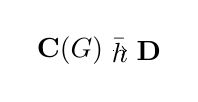
\begin{tikzpicture}
  \node (CG) {${\bf C}(G)$};
  \node (D) [right of=CG] {${\bf D}$};
  \draw[->, dotted] (CG) to node {$\bar h$} (D);
 \end{tikzpicture}
 \end{center}

 ${\bf Graphs}$において:
 \begin{center}
 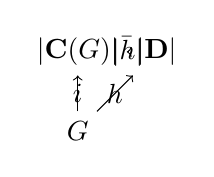
\begin{tikzpicture}
  \node (CG) {$|{\bf C}(G)|$};
  \node (D) [right of=CG] {$|{\bf D}|$};
  \node (G) [below of=CG] {$G$};
  \draw[->] (CG) to node {$|\bar h|$} (D);
  \draw[->] (G) to node {$i$} (CG);
  \draw[->] (G) to node [swap]{$h$} (D);
 \end{tikzpicture}
 \end{center}
\end{UMPofFreeCat}

頂点を一つだけ持つグラフ上の自由圏は,単に辺の集合上の自由モノイドになる.
二つの頂点とその間にただ一つの辺のみを持つグラフ上の自由圏は有限圏${\bf
2}$ である.次の形のグラフ
\begin{center}
 \begin{tikzpicture}
  \matrix (m)[matrix of math nodes, column sep=2cm] {A & B\\};
  \path[->]
    (m-1-1.20) edge node {$e$} (m-1-2.160)
    (m-1-2.200) edge node {$f$} (m-1-1.340);
 \end{tikzpicture}
\end{center}
上の自由圏は,(恒等射の他に)無限に多くの射
\[
 e, f, ef, fe, efe, fef, efef, \ldots
\]
を持つ.
\index{けん@圏!しゆう@自由---|)}

\section{基礎論:大きい,小さい,局所的に小さい}
\label{sec:foundations}
\index{きそろん@基礎論|(}
次のふたつの事を区別するところから始めよう:

\begin{enumerate}
 \renewcommand{\labelenumi}{(\roman{enumi})}
 \item 数学の圏論的基礎付け
 \item 圏論の数学的基礎付け
\end{enumerate}

ひとつ目に関しては,圏論\index{けんろん@圏論}を
集合論\index{しゆうこうろん@集合論}に代わって「数学の基礎」を提供する道
具として用いることが出来る,ということをきいたことがあるかもしれない.そ
れこそが正に一つめに当てはまるケースだが,これから我々がやろうとしているこ
とではない.集合論では,「無限集合が存在する」などといった存在公理や,「ど
んな集合に対しても冪集合が存在する」といった導出公理を置くことから始めて,
「全数学」を展開するのに原理的に十分な数学的対象(つまり集合)の宇宙を構
成する.我々の,どんな射もドメインとコドメンを持つという圏論の公理は,ど
んな集合に対しても冪集合が存在する,といったような公理とは異なった理解が
必要である!では,違いはなにか.集合論では——少なくとも通常考えられてい
る範囲では——公理は特定のたった一つの集合宇宙に言及する(或いは決定する)
ものと見做されている.対照的に,圏論の公理は何か(すなわち圏)の
{\bfseries 定義}である.これはちょうど,群論や位相空間論の公理系が,興味のあ
る対象の定義として使われているのと同じことである.一方,こういった体系
では,「背景」や「基礎」となる体系,たとえば集合論や型理論などの存在を仮
定している.こうした集合の理論を,一方で,圏論や他の方法によって決定する
ことも可能である.

こうしてやっと,二つめの議論へと辿り着く.我々は,これからの議論では他の
数学的対象と同じく圏も集合と写像を用いて何らかの形で表わされているとする.
そして,圏論的(あるいは他の)方法による数学の基礎付けもありうる,という
注意を気に留めておくにとどめよう.しかし,圏論ではしばしば集合論上の困難
に遭遇することがよくある.それは主に大きさの問題である.いくつかの圏は,
集合論の枠組みで捉えるには「大きすぎる」のだ.この問題は
第\ref{sec:free categories}節で Cayley 表現について考察した際に既に遭遇
している.その際は対象となる圏の射の集まりが集合であることを条件として課
したのであった.一般的に,そうした制限を(群論などでもあるように)あまり
気にせずに済ませたいが,たとえば
「圏」$\Sets$\index{Sets@$\Sets$}ですらちゃんとした圏にはならず,それは
これから考察してゆく幾つもの圏についても同様なのである.

こうした問題に対処する形式的な手法は色々とあり,Mac Lane の本で議論さ
れている.我々の目下の目的では,次の区別が便利である.

\begin{definition}
 圏${\bf C}$が{\bfseries 小さな圏}
 \index{けん@圏!ちいさな@小さな---|textit}であるとは,対象の集まり
 ${\bf C}_0$,射の集まり ${\bf C}_1$がともに集合である
 ことである.そうでない場合,${\bf C}$ は{\bfseries 大きな圏}
 \index{けん@圏!おおきな@大きな---|textit}であるという.
 \index{おおきなけん@大きな圏|see{圏, 大きな}}
 \index{ちいさなけん@小さな圏|see{圏, 小さな}}
\end{definition}
たとえば,全ての有限圏は明らかに小さな圏であり,全ての有限集合と写像の
圏$\Sets_{\rm fin}$も小さな圏である.(実際には,どの集合も他の有限集合
のみからなること,つまり「遺伝的に有限である」という条件が必要となる.)
一方で,posetのなす圏$\Pos$や群の圏${\bf Group}$,すべての集合の圏$\Sets$
\index{Sets@$\Sets$}は全て大きな圏である.$\Cat$ は小さな圏全体からなる
圏であるとすると,それ自身は大きな圏となる.したがって,特に,$\Cat$はそ
れ自身の対象とはならないので,ある読者は安心するだろう.

しかし,これでも全ての問題が解決されたわけたわけではない.例えば,大きな
圏 ${\bf Group}$と$\Sets$について,一方から他方への函手全体からなる圏
といった構造について後程考察しようとする(この「函手圏」は後で定義され
る).しかし,こうした圏は小さくないので,これらを一般的な集合論で直接的
に扱うことは出来ない(圏が「大きすぎ」てしまう).したがって,こうした構
造を扱うためには,更に洗練された「クラス」の理論が必要となる.これが単に
技術的な基礎の問題に過ぎない場合については特に気にしないことにする(Mac
Lane 本 I.6 節がこの問題を取り扱っている).一方,次の概念はこの問題と
関連する概念のなかでもとても便利な概念である.

\begin{definition}
 圏 ${\bf C}$ が{\bfseries 局所的に小さい}
 \index{けん@圏!きよくしよてきにちいさな@局所的に小さな---|textit}
 とは,${\bf C}$の任意の対象 $X, Y$について,集まり
 $\Hom_{\bf C}(X, Y) = \set{f \in {\bf C}_1 | f: X \to Y}$
 が{\bfseries 集合である}ことである(このとき $\Hom_{\bf C}(X, Y)$
 は{\bfseries Hom集合}と呼ばれる).
 \index{きよくしよてきにちいさなけん@局所的に小さな圏|see{圏, 局所的に小さな---}}
\end{definition}
事実,我々が考察する大きな圏の多くは局所的に小さな圏である.$\Sets$ は
$\Hom_{\Sets}(X,Y) = Y^X$ でありこれは$X$から$Y$への写像全体の
{\bfseries 集合}であるので小さな圏である.同様に,$\Pos$
\index{Pos@$\Pos$}, ${\bf Top}$\index{Top@${\bf Top}$},
${\bf Group}$\index{Group@${\bf Group}$}なども局所的に小さな圏であり
($\Cat$はどうか?),また任意の小さな圏はもちろん局所的に小さな圏である.

\begin{warn}
 {\bfseries 小さな}圏と{\bfseries 具体}圏を混同してはいけない.圏が具体
 圏であるとは,対象が何らかの(構造の入った)集合で,射が(或る種の)写
 像であることである.圏の{\bfseries 全ての対象の集まり}と全ての射の集ま
 りが集合であるとき,圏は小さな圏であると呼ばれた.実数全体$\R$は poset
 圏と見做せば小さな圏だが具体圏ではない.全てのposetからなる圏$\Pos$は具
 体圏だが小さくない.
\end{warn}
\index{きそろん@基礎論|)}
\section{演習問題}
\begin{enumerate}
 \item $\Rel$\index{Rel@$\Rel$}の対象は集合,射$A \to B$は$A$から$B$への
       二項関係,即ち$R \subseteq A \times B$ である.集合$A$上の恒等射
       は,同値関係 $\set{\langle a, a\rangle \in A\times A | a \in A}$
       とする.また,$\Rel$での射の合成は,
       \[
	S \circ R = \set{\langle a, c\rangle \in A \times C | \exists
       b\,(\langle a, b\rangle \in R\; \&\; \langle b, c\rangle \in S)}
       \]
       で定める.但し$R \subseteq A \times B$, $S \subseteq B
       \times C$ とする.
       \begin{enumerate}
	\item $\Rel$ が圏であることを示せ.
	\item 次に,対象はそれ自身に,写像 $f: A \to B$をそのグラフ,
	      \[
	       G(f) = \set{\langle a, b\rangle \in A \times B | a \in A}
	      \]
	      に移す函手 $G: \Sets \to \Rel$ が存在することを示せ.
	\item 最後に,各関係$R \subseteq A \times B$ を,次で定められる逆
	      関係 $R^c \subseteq B \times A$ に移す函手 $C: \Rel^{\rm
	      op} \to \Rel$ が存在することを示せ.
	      \[
	       \langle a, b \rangle \in R^c \iff \langle b, a\rangle \in R
	      \]
       \end{enumerate}
 \item 次の圏同型\index{とうけい@同型}がそれぞれ成立するかどうか考察せよ.
       \begin{enumerate}
	\item $\Rel \cong \Rel^{\rm op}$
	\item $\Sets \cong \Sets^{\rm op}$
	\item 集合 $X$ を一つ固定する.$\Pow(X)$を包含関係につい
	      ての poset圏とみなす($\Pow(X)$の射は,任意の $A, B
	      \subseteq X$に対して部分集合の包含関係$A\subseteq B$
	      である).このとき,$\Pow(X) \cong \Pow(X)^{\rm op}$か?
       \end{enumerate}
 \item \begin{enumerate}
	\item $\Sets$の同型射\index{とうけいしや@同型射}は全単射と一致
	      することを示せ.
	\item ${\bf Monoids}$の同型射は全単射準同型写像と一致すること
	      を示せ.
	\item $\Pos$での同型射は全単射単調写像とは一致{\bfseries
	      しない}ことを示せ.
       \end{enumerate}
 \item $X$ を位相空間とし,特殊化順序
       \index{いそうのとくしゆかしゆんしよ@位相の特殊化順序}によって各点
       にプレ順序が入っているものとする.即ち, $y$ が $x$ を含む開集合
       に必ず含まれているとき,その時に限り $x \leq y$ とする.このとき,
       これがプレ順序となっていることを示し,$X$ が $T_0$空間(任意の異
       なる二点について,どちらか一方を含みもう一方を含まないような開集合が存在
       する)のとき $X$ は poset となることを示せ.また,$X$ が $T_1$空
       間(任意の異なる二点に対し,一方を含み他方を含まないような開集合
       がそれぞれの点に対し存在する)であるとき,順序は自明となることを示せ.
 \item 任意の圏 ${\bf C}$ に対し,対象$C$上のスライス圏から${\bf C}$ への,
       「$C$を忘れる」函手 $U: {\bf C}/C \to {\bf C}$ を定義せよ.更に,
       ${\bf dom} \circ F = U$ となる函手 $F: {\bf C}/C \to {\bf C}^{\to}$
       を見付けよ.
 \item 圏${\bf C}$の対象$C$下の「コスライス圏」$C/{\bf C}$ を,スライス
       圏 ${\bf C}/C$ と「双対圏」をとる操作 $-^{\rm op}$ を使って構成せ
       よ.
 \item $2 = \{a, b\}$ を異なる二つの元$a, b$ からなる任意の集合とする.
       函手 $F: \Sets/2 \to \Sets \times \Sets$ を
       $F(f: X \to 2) = (f^{-1}(a), f^{-1}(b))$で定める.これは圏の同型
       射となっているか?また,$2$ではなく一点集合 $1 = \{a\}$ の場合
       はどうか?
 \item 任意の圏${\bf C}$は,二項関係 $\leq$ を次で定めることでプレ順序
       $P({\bf C})$を決定する.
       \begin{center}
	射 $A \rightarrow B$ が存在するとき,その時に限り $A \leq B$
       \end{center}
       このとき,$P$ が函手を定めることを,$P$の函手に対する動作を定義し
       函手の条件を満たすことを確かめることによって示せ.また,$P$ がプ
       レ順序集合を圏に埋め込む自明な函手の(片側)逆射になっていること
       を示せ.
 \item 次のグラフ\index{くらふ@グラフ}上の自由圏を,対象・射・合成を与え
       ることで説明せよ.
       \begin{enumerate}
	\item  
	      
	       \begin{center}
		\begin{tikzpicture}
		 \matrix (m)[matrix of math nodes, column sep=2cm] {
		 a & b\\
		 };
		 \path[->] (m-1-1) edge node {$e$} (m-1-2);
		\end{tikzpicture}
	       \end{center}
	\item  
	      
	       \begin{center}
		\begin{tikzpicture}
		 \matrix (m)[matrix of math nodes, column sep=2cm] {
		 a & b\\
		 };
		 \path[->] (m-1-1.20) edge node {$e$} (m-1-2.160)
		           (m-1-2.200) edge node {$f$} (m-1-1.340);
		\end{tikzpicture}
	       \end{center}
	\item  
	      
	       \begin{center}
		\begin{tikzpicture}
		 \matrix (m)[matrix of math nodes, column sep=2cm, row
		 sep=2cm]
		 {
		 a & b\\
		   & c\\
		 };
		 \path[->]
		   (m-1-1) edge node {$e$} (m-1-2)
		           edge node {$g$} (m-2-2)
		   (m-1-2) edge node {$f$} (m-2-2);
		\end{tikzpicture}
	       \end{center}
	\item  
	      
	       \begin{center}
		\begin{tikzpicture}
		 \matrix (m)[matrix of math nodes, column sep=2cm, row
		 sep=2cm]
		 {
		 a & b\\
		   & c\\
		 };
		 \path[->]
		   (m-1-1.20) edge node {$e$} (m-1-2.160)
		   (m-1-2.200) edge node {$h$} (m-1-1.340)
		   (m-2-2) edge node {$g$} (m-1-1)
		   (m-1-2) edge node {$f$} (m-2-2);
		\end{tikzpicture}
	       \end{center}
       \end{enumerate}
 \item 射をちょうど6本持つ自由圏\index{けん@圏!しゆう@自由---}はいくつある
       か?それらを生成するグラフ\index{くらふ@グラフ}を描け.
 \item 自由モノイド函手
       \[
	M: \Sets \to \Mon
       \]
       が存在することを,次の二通りの方法で示せ.
       \begin{enumerate}
	\item 特に $M(X) = X^*$ として,その写像 $f: A \to B$ への作用
	      \[
	       M(f): M(A) \to M(B)
	      \]
	      を,
	      \[
	       M(f)(a_1\ldots a_k) = f(a_1)\ldots f(a_k),\ \ \
	      a_1,\ldots a_k \in A
	      \]
	      で定義せよ.
	\item 自由モノイドの普遍写像性のみを仮定して,それを用いて函手の写
	      像への効果を決定し,これが函手となることを示せ.
       \end{enumerate}

       上の二つの方法が互いにどう関係しているかを比較せよ.
 \item 射を辺の列として定義したグラフ上の自由圏
       \index{けん@圏!しゆう@自由---}の普遍写像性を確かめよ.
       特に,${\bf C}(G)$をグラフ$G$上の自由圏とし,グラフ準同型
       $i: G \to U({\bf C}(G))$を,$G$の辺・頂点を,${\bf C}(G)$の対応す
       る射・対象に移すものとする.このとき,任意の圏 ${\bf D}$ とグラフ
       準同型 $h: G \to U({\bf D})$ に対し,函手
       \[
	\bar h: {\bf C}(G) \to {\bf D}
       \]
       が一意に存在し,
       \[
	U(\bar h) \circ i = h
       \]
       となることを示せ.ここで,$U: \Cat \to {\bf Graph}$は台グラフ函手
       である.
 \item Cayley 表現を用いて,任意の小さな圏は,対象が集合で射がその間の
       写像であるような「具体圏」と同型であることを示せ.
 \item 圏の概念は,射と対象という二つの構成要素によらずとも,ただひとつ
       の要素,すなわち射のみによって定義することもできる.ドメイン・コ
       ドメインは,部分的に定義された合成演算に対し単位的に振る舞う射と
       して定義される.これに関するMac Lane『圏論の基礎』I.1 節の定義を
       読み,そこで言及されている練習問題を解いて二つの定義の同値性を示
       せ.
\end{enumerate}
